\documentclass[12pt]{article}
%\usepackage{amsrefs}
\usepackage{fullpage}
\usepackage{enumerate}
\usepackage{multicol}
\usepackage{comment}
\usepackage{lastpage}
\usepackage{fancyhdr}
\pagestyle{fancy}

\addtolength{\topmargin}{-0.25in}
\usepackage{graphicx}	
\usepackage{array, multicol}
\usepackage{amsmath,amsfonts}

\everymath{\displaystyle}
\renewcommand*{\thefootnote}{\fnsymbol{footnote}}

\fancypagestyle{plain}{
	\fancyhf{}
	\addtolength{\headheight}{2.92\baselineskip}
	\lhead{\bf MATH 2574 (Calculus III) \\
		Fall 2015 \\
		}
	\rhead{{Name:} \underline{\hspace{40ex}} \\
		\vspace{0.75pc}
		{Drill:} \underline{\hspace{40ex}} \\
		\vspace{0.5pc}
		Tues 3 Nov 2015}
	\rfoot{Quiz 9 p.\thepage\ (of \pageref{LastPage})}
	}
\fancyhf{}
\renewcommand{\headrulewidth}{0pt}

\title{\flushleft\vspace{-2.5pc}\Large
	\bf Quiz 9: The Jacobian (\S13.4-13.5,\ 13.7)}
\author{}
\date{}

\rfoot{Quiz 9 p.\thepage\ (of \pageref{LastPage})}

% % % % %
\begin{document}
\maketitle

\vspace{-4pc}
%\noindent{\bf Directions:} You may collaborate.  
%
%\vspace{1pc}
The Jacobian is a magnification (or reduction) factor that relates the area of a small region, or neighborhood, near a point $(u,v)$ in $\mathbb R^2$ ($uv$-plane), to the area of the \textit{preimage}\footnote{
	The text instead uses the term \textit{image} and writes $T(S)=R$.  The reason for the discrepancy is delicate and relevant to the field of Algebraic Geometry.  The transformation $T$ can be described in two ways:
	\begin{align*}
	T:\left\{\text{ unknowns in the $x$s and $y$s }\right\} &\to \left\{\text{ unknowns in the $u$s and $v$s }\right\} &\quad \text{\it (Algebraic Paradigm)} \\
		&\text{ or } & \\
	T:\left\{\text{ known values in the $u$s and $v$s }\right\}	&\to \left\{\text{ corresponding $x$- and $y$-values }\right\} & \text{\it (Geometric Paradigm)}
	\end{align*} 
} of that region near the point $(x,y)$ in $\mathbb R^2$ ($xy$-plane), where 

\vspace{-1pc}
\[
T:x=g(u,v)\quad \text{and}\quad y=h(u,v)
\]

\vspace{-0.5pc}
\noindent is a one-to-one transformation.   
\vspace{1pc} 

Suppose $S$ is a little rectangle in the $uv$-plane with vertices $(0,0),(\Delta u,0),(\Delta u,\Delta v),(0,\Delta v)$.  The preimage of $S$ under the transformation given above is a small region $R$ in the $xy$-plane.  The arrows $(\mapsto)$ below, and the picture, indicate the respective preimages of each of the following points:
\vspace{-0.75pc}
\[\begin{split}
(0,0)=O & \mapsto O'%=\left(g(0,0),h(0,0)\right) 
\\
(\Delta u,0)=P & \mapsto P'%=\left(g(\Delta u,0),h(\Delta u,0)\right) 
\\
(0,\Delta v)=Q & \mapsto Q'%=\left(g(0,\Delta v),h(0,\Delta)\right)
\end{split}\]

\vspace{-1.5pc}
\begin{center}
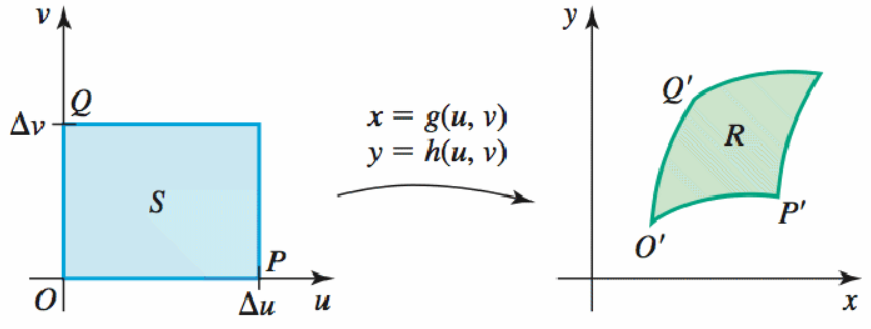
\includegraphics[scale=0.75]{Q9pic}
\end{center}

\begin{enumerate}[(a)]
\item {\bf (3 pts)} 
Write down the coordinates for each of the points $O',P',Q'$.
\[\begin{split}
O' &= \hspace{40ex} \\[1pc]
P' &= \hspace{40ex} \\[1pc]
Q' &= \hspace{40ex}
\end{split}\]

% % %
\newpage
\item The linear approximation of $g(u,v)$ near the point $O=(0,0)$ is:  
\vspace{-0.5pc}
\[
\textstyle g(u,v)\approx g(0,0) + g_u(0,0)\cdot u%\left.\dfrac{\partial g}{\partial u}\right|_{(0,0)} + v\left.\dfrac{\partial g}{\partial v}\right|_{(0,0)}
+ g_v(0,0)\cdot v
\] 

\begin{enumerate}[i. ]
	\item {\bf (1 pt)} Write down the linear approximation of $h(u,v)$ near $O$.
	\vspace{3pc}
	
	\item {\bf (2 pts)} The points $P$ and $Q$ are close to the point $O$; use the linear approximations for $g$ and $h$ to compute 
	\[\begin{split}
	g(\Delta u,0) \approx \hspace{30ex} h(\Delta u,0) \approx &	\hspace{25ex} \\[1.75pc]
	g(0,\Delta v) \approx \hspace{30ex} h(0,\Delta v) \approx &
	\end{split}\]
	\vspace{0.5pc}
	
	\item {\bf (2 pts)} Use the approximations in ii. to find the area of the parallelogram with sides given by the vectors $\overrightarrow{O'P'}$ and $\overrightarrow{O'Q'}$.  {\it (Hint: Use the cross product by first adding a third variable and setting its direction equal to zero.)}
	\vspace{22pc}
	
	\item {\bf (2 pts)} What is the approximate ratio of the area of $R$ to the area of $S$?

	\end{enumerate}

\end{enumerate}
% % % % %
\end{document}